\documentclass{article}
\usepackage[T1]{fontenc}
\usepackage{lmodern}
\usepackage{graphicx}
\usepackage{amsmath,amssymb}
\usepackage[a4paper,margin=2cm]{geometry}
\usepackage[absolute,overlay]{textpos}
\setlength{\TPHorizModule}{1mm}
\setlength{\TPVertModule}{1mm}
\usepackage[indonesian]{babel}
\usepackage{hyperref}
\setlength{\emergencystretch}{2em}
% unit: Halaman 13

\begin{document}

% === Halaman 13 (llm) ===

Alice \vspace{5mm} Bob \vspace{5mm} Rinaldi M/II4020 Kriptografi

\vspace{117.02mm}

% deskripsi: Diagram pertukaran kunci Diffie-Hellman yang menunjukkan langkah-langkah perhitungan Alice dan Bob menggunakan parameter publik g dan p untuk menghasilkan kunci rahasia bersama K.
% bbox normalisasi: [0.1610, 0.5300, 0.8380, 0.9240]
\begin{textblock*}{142.17mm}(33.81mm,157.41mm)
\noindent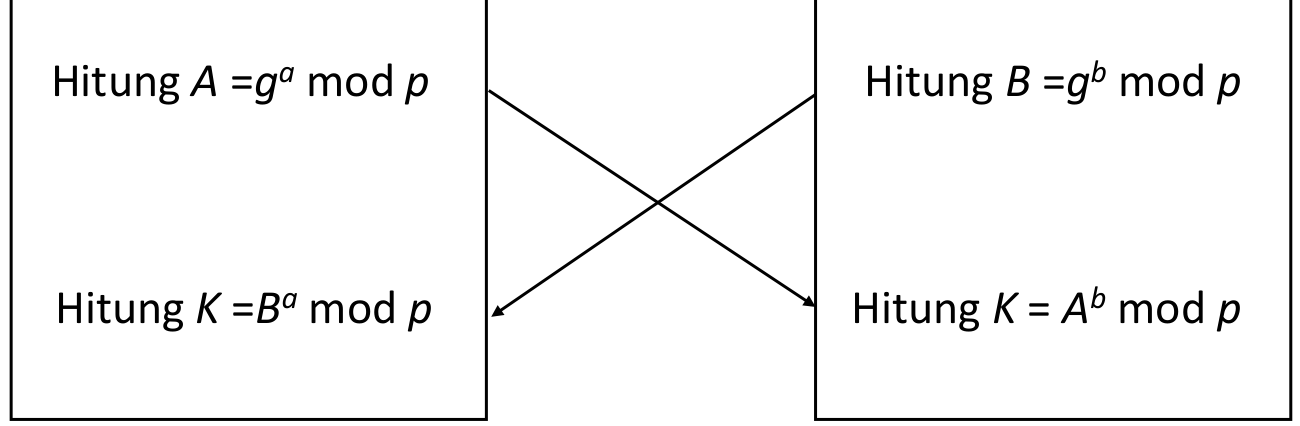
\includegraphics[width=142.17mm,height=117.02mm]{../../images/llm/page_013_img_01.png}%
\end{textblock*}

\end{document}
